\begin{figure}[t!]
\centering
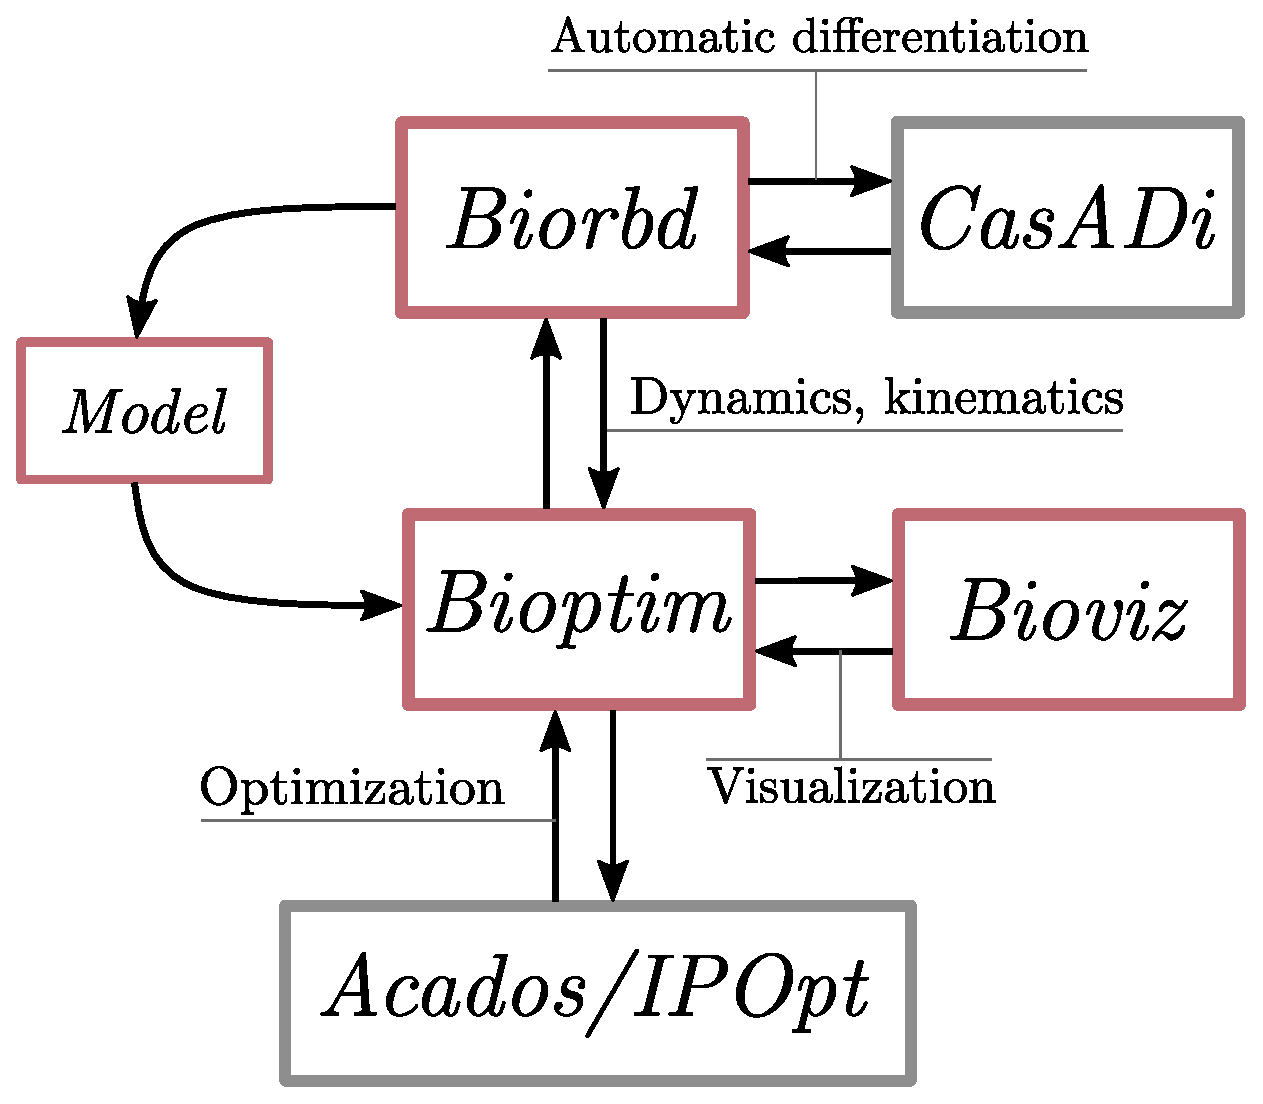
\includegraphics[width=0.9\columnwidth]{figures/dependencies.eps}
\caption{\bioptim dependencies flowchart. The red-boxed software are developed by the S2M team.}
\label{fig:dependencies}
\vspace*{-0.5cm}
\end{figure}


\subsection{Implementation and dependencies}
\bioptim is the top layer of a succession of software on which it depends to perform various calculations (\textit{Biorbd}: dynamics; \textit{CasADi}: automatic differentiation; \textit{IPOpt, Acados}: optimization; \textit{Bioviz}: visualization).
Within this software bundle, Bioptim's main role is to shape the problem in order to allow its dependencies to communicate efficiently, while providing an intuitive and flexible interface to the user (Fig.~\ref{fig:dependencies}).
Therefore, it was chosen to be written in Python for its flexibility and its widespread use among researchers.
However, all intensive calculations behind the interface are performed in C or C++, keeping \bioptim both fast and easy to customize.

\subsection{Design}
\`bioptim shapes and solves optimal control problems whose two required entries are a model (.\textit{bioMod} file) and an OCP.
 
The model file contains the geometrical characteristics, the mass and inertia parameters, the geometrical markers and possibly the muscular information of the model. 
It also allows the user to design or import meshes for visualization purposes.

The OCP is implemented as a succession of nonlinear problems (NLPs), which allows the formulation of multi-stage OCPs. Each NLP has the following attributes: a dynamics type, a list of objective function, constraints, initial guesses, a number of shooting points and the duration of the problem.
Based on these inputs, \bioptim properly sets up the multiple shooting transcription of the OCP, with appropriate continuity constraints in the case of multiple NLPs, and shapes it up to feed the non-linear solver (Ipopt or Acados). 

\subsubsection{Dynamics types}
The dynamics type defines which variables are states ($\state$), which ones are controls ($\control$) and which ones are parameters ($\param$).
Then, it implements the ordinary differential equation governing the state transition:

\[
\dstate = f(\state, \control, \param).
\addtag
\label{eq:state_transition}
\]

\noindent Ten dynamics are implemented in \bioptim,
MUSCLE-EXCITATIONS-AND-TORQUE-DRIVEN, 
MUSCLE-ACTIVATIONS-AND-TORQUE-DRIVEN,
MUSCLE-ACTIVATIONS-DRIVEN,
MUSCLE-EXCITATIONS-AND-TORQUE-DRIVEN-WITH-CONTACT, 
MUSCLE-EXCITATIONS-DRIVEN,
MUSCLE-ACTIVATIONS-AND-TORQUE-DRIVEN-WITH-CONTACT,
TORQUE-DRIVEN,
TORQUE-ACTIVATIONS-DRIVEN, 
TORQUE-ACTIVATIONS-DRIVEN-WITH-CONTACT, 
TORQUE-DRIVEN-WITH-CONTACT.
(Est-ce utile de lister, Tableau ?).
Even if these dynamics types exhaustively span the current usages in biomechanics, a custom dynamics type is also pre-implemented to allow easy problem customization.

\subsubsection{Objective functions}
Accordingly to the optimal control formalism, there are two main types of objective functions, namely Lagrange and Mayer. Lagrange types are running objectives, integrated over the whole NLP. Mayer types are time-specific objectives. Classically, they correspond to a terminal objective, but to be more versatile, they can be defined at any instant in \bioptim.

These objective functions can depend on any of the optimization variable, \textit{i.e.} the controls, the states and the parameters. A lot of objective function types are already implemented in \bioptim ($>20$), among which tracking and minimizing objectives, on the states, the controls, geometrical markers, contact forces, etc. Should one go missing, a custom objective type is also pre-implemented.

When declaring the desired list of objective function for a given problem, each objective function type is associated with a weight, and the user can flexibly choose on which components of the vector variables the objective must apply. If applicable (for tracking objective functions mainly), the user must also specify the numerical target of the objective.

\subsubsection{Constraints}